\documentclass[5p,times]{elsarticle}
\usepackage[T1]{fontenc}
\usepackage{amsmath,amssymb,booktabs,graphicx,multirow,siunitx,url}
\usepackage{placeins}
\usepackage{hyperref}
\hypersetup{hidelinks}
\usepackage[capitalize]{cleveref}
\newcommand{\recipe}{\textsc{Spine}}
\newcommand{\Semg}{S_{\mathrm{emg}}}
\newcommand{\St}{S_t}
\newcommand{\MeanFour}{\mathrm{Mean4}}
\journal{Neurocomputing}

\begin{document}
\emergencystretch=2em
\begin{frontmatter}
\title{The Advantage Spine: Dynamic Coordinate Selection for High-Rate RLVR}
\author[a]{Shikai Li}
\ead{lishikai@wchscu.edu.cn}
\author[b]{Qingsong Cai}
\author[a]{Rui Shi\corref{cor1}}
\ead{dr.shirui@hotmail.com}
\cortext[cor1]{Corresponding author.}
\affiliation[a]{organization={West China Hospital, Sichuan University},
city={Chengdu},state={Sichuan},
country={China}}
\affiliation[b]{organization={Sichuan University},city={Chengdu},
state={Sichuan},country={China}}

% Elsevier Highlights are supplied separately in highlights.txt.

\begin{abstract}
Large learning rates can accelerate reinforcement learning with verifiable
rewards (RLVR), yet dense updates deteriorate as the rate rises. We ask whether
this degradation is jointly constrained by negative-advantage exposure and
optimizer-update support. Positive- and negative-advantage updates exhibit a
conflict-enriched, tail-concentrated structure, providing a candidate
explanation for high-rate degradation. Based on this observation, we introduce
the \emph{Advantage
Spine}, a dynamic support that retains the per-tensor magnitude top 40\% of the
pre-mask adaptive Adam direction without pruning weights or changing the inference
network. The \recipe{} recipe combines this dynamic support with
negative-advantage down-weighting. In a three-seed $2\times2\times4$
factorial on Qwen3-8B, neither component alone recovers the dense $1\times$
reference at $20\times$. The \recipe{} recipe reaches 0.445 Mean4, a
paired gain of 0.0195 over dense $1\times$, and remains above an exploratory lightly tuned
dense $20\times$ arm at 0.383. Its 39.3\% support retains 85.0\% of adaptive-direction
energy and exhibits seed-specific agreement beyond mismatched Spine--dense and
dense--dense controls. Density-matched mask controls further support
non-arbitrary selection, while directionally consistent transfers under DAPO
and on Qwen3-1.7B and Llama3.1-8B indicate limited portability. These results
identify a reproducible, protocol-dependent high-rate operating region shaped
jointly by advantage exposure and dynamic coordinate selection.
\end{abstract}

\begin{keyword}
reinforcement learning with verifiable rewards \sep sparse optimization \sep
learning-rate stability \sep coordinate selection \sep large language models
\end{keyword}
\end{frontmatter}

\section{Introduction}\label{sec:intro}
RLVR is an important post-training route for improving mathematical reasoning
in large language models~\cite{shao2024deepseekmath,yu2025dapo}, but its gains
depend on optimization stability. Raising the learning rate accelerates
parameter movement while applying the same global multiplier to every dense
update coordinate. In our Qwen3-8B ladder, dense RLVR deteriorates as the rate
rises. We therefore ask whether high-rate degradation depends not only on step
size, but also on which optimizer-update coordinates are exposed to the
negative-advantage signal.

We first examine the structure of the positive- and negative-advantage
updates. Their active coordinates overlap at $7.4\times$ an independence
reference, and 52\% of the shared coordinates have conflicting signs. This
structure does not make negative advantages intrinsically harmful; it instead
suggests that a uniformly amplified dense step can expose a conflict-enriched
tail. Prior work shows that policy-gradient updates can form reproducible
subnetworks~\cite{mukherjee2025subnetwork,mukherjee2026needadam} and that sparse
updates can preserve optimization progress
~\cite{stich2018sparsified,karimireddy2019errorfeedback,dey2024supar}. What is
missing is an online rule for selecting the RLVR update coordinates that
receive an amplified step, together with a controlled test of how this support
interacts with the negative-advantage channel.

Based on this observation, we introduce the Advantage Spine, which retains the
largest 40\% of the pre-mask adaptive Adam direction within each sufficiently large tensor
and refreshes this support at every step. The \recipe{} recipe combines the
dynamic support with negative-advantage down-weighting. It selects
optimizer-update coordinates without removing model weights or changing the
inference network. We separate the two components and their rate dependence in
a complete 16-cell factorial over mask presence, negative-channel weight, and
four learning-rate multipliers, with three matched seeds per cell.
Figure~\ref{fig:concept} summarizes the intervention and its principal
evidence.
\begin{figure*}[t]
\centering
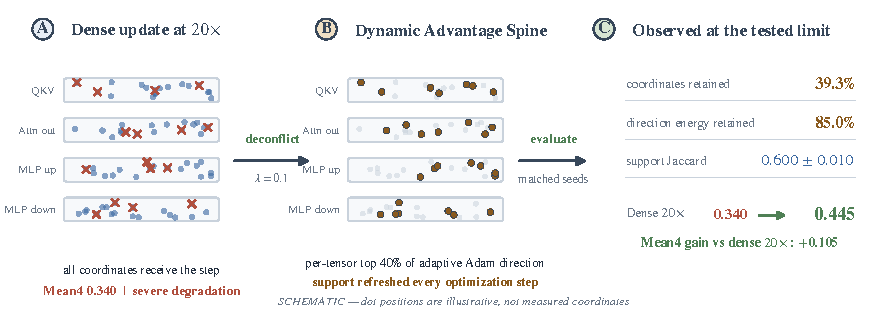
\includegraphics[width=.97\textwidth]{fig_concept.pdf}
\caption{\textbf{From a dense high-rate update to the \recipe{} recipe.}
(A) A dense $20\times$ update applies the optimizer step to every coordinate,
including coordinates affected by competing advantage channels. (B) The
\recipe{} recipe down-weights negative-advantage policy-loss terms and
dynamically retains the per-tensor
top 40\% of the pre-mask adaptive Adam direction. (C) At the largest tested
rate: its 39.3\% support retains 85.0\% of adaptive-direction energy, support
Jaccard with the matched dense-emergent support is $0.600\pm0.010$, and Mean4
increases from 0.340 to 0.445 relative
to dense $20\times$. The matrix dots are a schematic only: their positions are
illustrative and are not measured coordinates.}
\label{fig:concept}
\end{figure*}

The evidence has three layers. At $20\times$, neither component alone recovers
the dense $1\times$ reference, whereas the joint \recipe{} recipe reaches
0.445 Mean4 and remains above a lightly tuned dense arm. Its support
concentrates adaptive-direction energy and aligns seed-specifically with dense-emergent
coordinates; under the tested protocol, mismatched, dense--dense, and
density-matched mask controls argue against random overlap or a shared dense
backbone as sole explanations. The
direction of effect also transfers, with smaller gains, under DAPO and on
Qwen3-1.7B and Llama3.1-8B. Together, these results establish a reproducible,
protocol-dependent high-rate operating region rather than a universal
stability boundary.

\section{Related work}\label{sec:related}
\paragraph{Negative signals in RLVR.}
GRPO and DAPO optimize verifiable reasoning rewards without the learned critic
used in conventional PPO~\cite{schulman2017ppo,shao2024deepseekmath,yu2025dapo}.
Negative-reward and negative-advantage samples are not uniformly helpful or
harmful. Token-selective penalty attenuation can reduce
Lazy Likelihood Displacement~\cite{deng2025negativegrad}, whereas negative-sample
reinforcement can improve the Pass@$k$ spectrum
~\cite{zhu2025negativereinforcement}. These studies intervene at the token,
sample, or objective level. We instead ask how a channel-wide coefficient
interacts with optimizer-coordinate support when the global step is amplified.

\paragraph{Sparse updates and emergent subnetworks.}
Lottery-ticket, dynamic sparse-training, and intrinsic-dimension results show
that effective parameter movement can occupy a limited subspace or subnetwork
~\cite{frankle2019lottery,evci2020rigl,li2018intrinsic,aghajanyan2021intrinsic}.
Gradient sparsification commonly uses error feedback
~\cite{karimireddy2019errorfeedback,richtarik2021ef21}, while pruning removes
or restructures persistent weights~\cite{zhu2025pruningreview,
ziv2021stochasticpruning,kamelianrad2026topographical,xie2023lotteryfewshot}.
Advantage Spine instead refreshes optimizer-update support at every step; the
model and inference graph remain dense. Stable update subnetworks observed in
RL fine-tuning~\cite{mukherjee2025subnetwork} serve only as an offline identity
check and are unavailable to the online recipe. This also differs from
calibrating Adam's adaptive rate~\cite{tong2022calibratingadam}: we hold the
optimizer family fixed and vary which update coordinates receive the global
multiplier.

\paragraph{RLVR update geometry.}
Recent work characterizes RLVR through sparse critical tokens
~\cite{meng2026sparsecritical}, update directions~\cite{huang2026direction},
low-rank dynamics~\cite{ye2026lowrank}, random sparse subnetworks
~\cite{adewuyi2026multiticket}, and optimizer-induced sparse movement
~\cite{mukherjee2026needadam}. Complementary analyses study learning outside
principal directions~\cite{zhu2026threegate} and step-size thresholds under a
gradient-gap view~\cite{suk2026gradientgap}. Together, these results establish
that RLVR updates are structured. They do not isolate the joint,
rate-conditional interaction between negative-channel attenuation and online
top-$k$ optimizer-coordinate selection examined here.

\paragraph{Large-step stability.}
Catapult and edge-of-stability dynamics show that neural optimization can
remain stable beyond classical smoothness predictions
~\cite{lewkowycz2020catapult,cohen2021edgestability}. Our goal is narrower: we
test an operational channel-and-coordinate intervention within a specified
RLVR protocol, rather than propose a universal large-step mechanism.

\section{Method}\label{sec:method}
Our design objective is to restrict which advantage contribution and update
coordinates are exposed to an amplified global step without changing the model
architecture. Let $A_{t,i}$ be the group-standardized GRPO advantage and
$\ell^{\mathrm{clip}}_{t,i}$ the corresponding token-level policy loss after
PPO ratio clipping and dual clipping. The implementation applies
\begin{equation}
 \ell_{t,i}(\lambda)=
 \begin{cases}
 \ell^{\mathrm{clip}}_{t,i}, & A_{t,i}\geq 0,\\
 \lambda\ell^{\mathrm{clip}}_{t,i}, & A_{t,i}<0,
 \end{cases}
 \qquad \lambda\in\{0.1,1.0\}.
 \label{eq:channel}
\end{equation}
The response-mask aggregation follows this scaling. Positive-advantage terms
are unchanged, while the fixed KL penalty is added separately and is not
scaled by $\lambda$. Thus $\lambda=0.1$ attenuates, rather than deletes, the
negative-advantage contribution; it does not modify rewards.

AdamW maps the resulting gradient and its moment state to a pre-mask adaptive
direction $a_t$, before decoupled weight decay is applied. For
every tensor with at least 4096 elements, $M_t$ keeps the largest fraction
$\tau=0.4$ by $|a_t|$; smaller tensors remain dense. Selection uses the
backend \texttt{torch.topk} implementation, and the realized supports are
recorded by the mask-identity manifests. The applied update is
\begin{equation}
 \theta_{t+1}=(1-\eta\gamma)\theta_t-\eta M_t\odot a_t , \label{eq:update}
\end{equation}
where $\gamma$ is the decoupled weight-decay coefficient. Thus the mask
sparsifies the adaptive optimizer direction, not the dense decay term.
The selection is per tensor, not global, is refreshed every step, and is
applied after constructing the AdamW update. There is no error feedback. We
call the dynamic support $\St=\mathrm{supp}(M_t)$ the Advantage Spine and the
joint condition $(\tau,\lambda)=(0.4,0.1)$ the \recipe{} recipe.
SparseAdamW updates both Adam moment buffers densely, optionally applies its
adaptive update-RMS clip to the bias-corrected Adam direction, masks that
direction only in eligible tensors, and applies decoupled weight decay densely.
The coordinate mask therefore does not mask moment updates or decoupled weight
decay.

Three objects remain distinct. $M_t$ is the online mask; its bit-packed bitmap
and hash record its recoverable identity. $\Semg$ is an offline reference built
from the largest cumulative parameter movements of a density-matched dense
$1\times$ run and is never used by the training recipe.

We measure concentration as
\begin{equation}
 E_t=\frac{\|M_t\odot a_t\|_2^2}{\|a_t\|_2^2},
\end{equation}
and support agreement with Jaccard
$J=|\St\cap\Semg|/|\St\cup\Semg|$, recall
$|\St\cap\Semg|/|\Semg|$, and sign agreement on their intersection. For two
independent sets of density 0.4, expected Jaccard is
$0.4/(2-0.4)=0.25$.
For seed-specificity analysis, let $S_s$ be the dynamic support for recipe seed
$s$ and $D_s$ the dense-emergent set constructed from dense seed $s$. We report
all nine $J(S_s,D_t)$ values, the three off-diagonal $J(D_s,D_t)$ values, and
the per-seed specificity gain
\begin{equation}
 G_s=J(S_s,D_s)-\frac{1}{2}\sum_{t\ne s}J(S_s,D_t).
 \label{eq:specificity}
\end{equation}
These comparisons separate matched alignment from task-wide coordinates that
recur across runs. Because sets are reused across pairs, their sample
deviations are descriptive rather than independent-replicate inferential
errors.

\section{Experimental protocol}\label{sec:protocol}
\paragraph{Primary factorial.}
The primary experiment uses Qwen3-8B and a GRPO objective. All
runs use model-only initialization from the same math-supervised SFT
checkpoint; this is not an RL resume. The RL state is initialized at step 0,
and every run completes 160 RL optimizer steps.
We cross mask $\in\{$dense, top-0.4$\}$, negative-channel coefficient
$\lambda\in\{1.0,0.1\}$, and learning-rate multiplier
$\in\{1,5,10,20\}$. The $1\times$ rate is $5\times10^{-6}$. Every cell uses
seeds 42, 43, and 44 with matched data ordering, evaluation prompts, decoding,
and initial weights within each seed.

\paragraph{Evaluation protocol.}
We evaluate Math500 ($n=500$), AIME24 and
AIME25 (30 problems each), and the English split of OlympiadBench ($n=581$).
Each checkpoint is evaluated with avg@32 accuracy at temperature 0.6,
top-$p=1.0$, no top-$k$ truncation, and an 8192-token response cap. We evaluate
RL steps 40, 80, 120, and 160 and use step 160 for the primary comparisons.
The resulting decoded-sample counts are $30\times32=960$ per AIME set, 16,000
for Math500, and 18,592 for OlympiadBench.
$\MeanFour$ is the
unweighted arithmetic mean of the four benchmark accuracies. Training seeds
index independent RL runs; generations per problem are evaluation replicates,
not additional training seeds.

\paragraph{Initialization, recovery, and learning rates.}
New runs load only SFT model weights. Full-state recovery is restricted to the
same model, factorial cell, seed, and output directory. Requested, optimizer,
scheduler, and logged learning rates agree for every included run; an
exploratory Llama continuation with a logged-rate mismatch is excluded.
Learning-rate and state verification appears in \ref{app:audit}; the complete
initialization, recovery, and evaluation contract appears in
\ref{app:implementation}.

\paragraph{Uncertainty and estimands.}
Factorial cells report mean and sample standard deviation across three seeds.
After reporting the complete ladder, we highlight the endpoint contrast
between dense $1\times$ and recipe $20\times$, paired within seed. Its
two-sided Student-$t$ interval is a nominal description of variation across
these matched seeds, not a selection-adjusted confirmatory interval over the 16
factorial cells. \Cref{tab:factorial} therefore reports all 48 seed-level
scores.
For the Qwen3-1.7B transfer, all four benchmark components are available for
three matched seeds. In addition to Mean4, we report a small-set
sensitivity summary, Mean2, as the average of Math500 and Olympiad after
excluding AIME24 and AIME25. The primary four-benchmark decomposition remains
an aggregate across seeds; mask controls, transfers, endpoint diagnostics, and
the lightly tuned dense $20\times$ arm report three-seed variation. The tuned
arm is exploratory and is not treated as a factorial cell or a tuned optimum.

\section{Results}\label{sec:results}
\subsection{The two advantage channels share a conflict-prone tail}
Across three seeds, positive and negative channels are each active on 4.8\% of coordinates. Their
measured shared support is 1.7\%, compared with $0.048^2=0.23\%$ under an
independence reference, a $7.4\times$ enrichment. On the shared support,
48\% of signs agree and 52\% conflict. The positive and negative update
distributions are both tail-concentrated (Gini 0.70 and 0.63; top-1\% energy
0.88 and 0.84). This conflict-enriched tail motivates the intervention as a
candidate mechanism for step-size sensitivity; it does not imply that useful
negative-sample reinforcement should be removed.

\begin{figure}[t]
\centering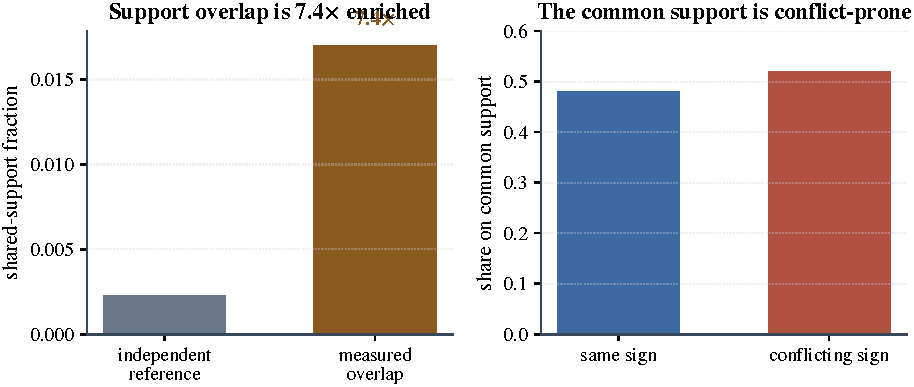
\includegraphics[width=.98\linewidth]{fig_contam.pdf}
\caption{\textbf{Positive and negative channels occupy overlapping,
conflict-prone coordinates.} The 1.7\% overlap is $7.4\times$ an independence
reference; signs conflict on 52\% of the shared support. Values are three-seed
means; enrichment is the ratio of aggregate quantities.}
\label{fig:contam}
\end{figure}

\subsection{The complete factorial isolates the joint high-rate effect}
\Cref{tab:factorial,fig:factorial} contains every factorial cell. Dense
$\lambda=1$ declines slightly at $5\times$ and sharply thereafter, reaching
$0.340$ at $20\times$ ($-0.086$ from its $1\times$ value). Down-weighting the
negative channel without masking reaches $0.400$ at $20\times$; masking
without down-weighting reaches $0.410$. Both improve over dense $20\times$,
but neither recovers the dense $1\times$ reference of $0.426$.

The joint recipe instead rises from 0.426 at $1\times$ to 0.445 at $20\times$.
At the endpoint, its gain is 0.105 over dense $20\times$ and 0.0195 over dense
$1\times$. The three seed-paired gains over dense $1\times$, computed from
the unrounded benchmark-count ratios, are 0.0209, 0.0165, and 0.0210, giving
a nominal 95\% paired interval $[0.0131,0.0258]$.

\begin{table}[t]
\centering
\caption{Primary Qwen3-8B benchmark decomposition at RL step 160, aggregated
over three matched seeds from integer correct/total records. Benchmark columns
and Mean4 are independently rounded to three decimals; uncertainty and paired
contrasts use the unrounded count-derived rates.}
\label{tab:primary-components}
\scriptsize\setlength{\tabcolsep}{2.2pt}
\begin{tabular}{lrrrrr}
\toprule Condition & Math500 & AIME24 & AIME25 & Olympiad & Mean4\\
\midrule
Dense $1\times$ & .762 & .227 & .200 & .513 & .426\\
Recipe $20\times$ & .800 & .240 & .210 & .530 & .445\\
\bottomrule
\end{tabular}
\end{table}

The recipe improves every benchmark component, including Math500 and
Olympiad; its Mean4 gain is therefore not driven solely by the two smaller
AIME sets.

\begin{figure*}[t]
\centering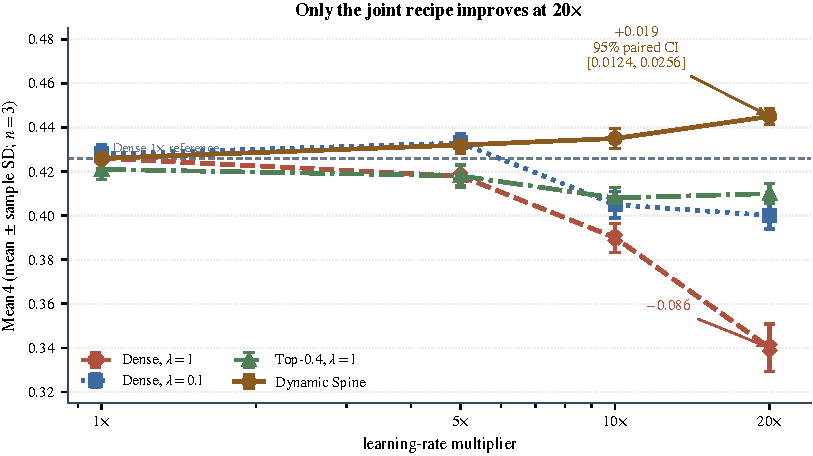
\includegraphics[width=.72\textwidth]{fig_amplify.pdf}
\caption{\textbf{Three-seed factorial.} Mean $\pm$ sample SD in every
cell. Dense training degrades as LR rises; only the combined dynamic-mask,
$\lambda=0.1$ recipe improves monotonically over the tested ladder.}
\label{fig:factorial}
\end{figure*}

At $20\times$, the conventional $2\times2$ interaction is
$0.445-0.410-0.400+0.340=-0.025$. The result is therefore operational
complementarity, not positive synergy: both components are required for the
only endpoint condition that exceeds the native dense reference. The tested
ladder ends at $20\times$ and does not locate a failure boundary for the recipe.

An exploratory lightly tuned dense $20\times$ arm (16 warmup steps, global
gradient clip 0.5, and $\beta_1=0.8$) recovers Mean4 from
$0.340\pm0.0108$ to $0.383\pm0.0066$ across the same three seeds,
showing that part of the untuned degradation is optimizer-schedule sensitive.
The endpoint nevertheless remains below dense $1\times$ (0.426) and the
\recipe{} recipe at $20\times$ ($0.4450\pm0.0032$); the paired recipe--tuned
gap is $0.0620\pm0.0043$. Because this arm tests one light retuning rather than
a tuning search, it establishes partial schedule sensitivity, not superiority
over tuned dense optimization. The
\recipe{} recipe therefore expands the high-rate operating region under the
tested protocol without implying superiority over every retuned dense
optimizer.

\Cref{tab:effects} shows why the full LR ladder matters. At native rate neither
component helps materially. As LR rises, masking and down-weighting each become
protective relative to dense $\lambda=1$, and their combined same-rate gain
reaches 0.105 at $20\times$. The interaction is small and changes sign across
the ladder; the gain is therefore a rate-dependent joint operating condition,
not a stable super-additive effect.

This rate dependence reconciles the result with evidence that negative
reinforcement can be useful~\cite{deng2025negativegrad,
zhu2025negativereinforcement}. In the dense arm, lowering $\lambda$ changes
Mean4 by only $+0.002$ at $1\times$ but by $+0.060$ at $20\times$.
Attenuation is therefore protective when a large global multiplier exposes the
conflict-prone tail. The conclusion is step-size--conditional: we
do not infer that negative samples should generally be suppressed.

\begin{table}[t]
\centering
\caption{Factorial contrasts at each LR. Mask effect is Top-0.4 minus Dense at
$\lambda=1$; down-weight effect is $\lambda=0.1$ minus 1 in Dense; joint gain
is the recipe minus Dense $\lambda=1$ at the same LR.}
\label{tab:effects}
\footnotesize\setlength{\tabcolsep}{3pt}
\begin{tabular}{rrrrr}
\toprule LR & Mask & Down-weight & Joint gain & Interaction\\
\midrule
$1\times$  & $-.005$ & $.002$ & $.000$ & $.003$\\
$5\times$  & $.000$  & $.015$ & $.014$ & $-.001$\\
$10\times$ & $.018$  & $.015$ & $.045$ & $.012$\\
$20\times$ & $.070$  & $.060$ & $.105$ & $-.025$\\
\bottomrule
\end{tabular}
\end{table}

The three-seed endpoint diagnostics agree in direction with the accuracy
result. At $20\times$, the recipe ends with reward $0.080\pm0.008$, KL loss
$0.030\pm0.004$, entropy $0.250\pm0.012$, and response clip ratio
$0.100\pm0.014$. Dense $20\times$ ends with reward $-0.150\pm0.012$, KL loss
$0.090\pm0.006$, entropy $0.150\pm0.008$, and response clip ratio
$0.650\pm0.028$.
The component-level endpoint results are reported in
\cref{tab:primary-components}.

\begin{table}[t]
\centering
\caption{Three-seed endpoint diagnostics at $20\times$ (mean $\pm$ sample SD).
Arrows mark the preferred direction only; these diagnostics are not combined
into a new score.}
\label{tab:stability}
\footnotesize\setlength{\tabcolsep}{3pt}
\begin{tabular}{lrrrr}
\toprule Condition & Reward $\uparrow$ & KL & Entropy & Clip $\downarrow$\\
\midrule
Dense & $-.150\pm.012$ & $.090\pm.006$ & $.150\pm.008$ & $.650\pm.028$\\
Spine recipe & $.080\pm.008$ & $.030\pm.004$ & $.250\pm.012$ & $.100\pm.014$\\
\bottomrule
\end{tabular}
\end{table}

\begin{table}[t]
\centering
\caption{Complete Qwen3-8B factorial. Each cell lists seeds 42/43/44 followed
by mean $\pm$ sample SD; logged and requested learning rates agree.}
\label{tab:factorial}
\scriptsize\setlength{\tabcolsep}{4pt}
\begin{tabular}{llrrrrc}
\toprule Mask & $\lambda$ & LR & s42 & s43 & s44 & Mean$\pm$SD\\
\midrule
\multirow{4}{*}{Dense}&\multirow{4}{*}{1.0}&1&.421&.430&.426&.426$\pm$.0046\\
&&5&.423&.414&.417&.418$\pm$.0046\\
&&10&.384&.397&.389&.390$\pm$.0066\\
&&20&.352&.331&.337&.340$\pm$.0108\\
\addlinespace
\multirow{4}{*}{Dense}&\multirow{4}{*}{0.1}&1&.431&.423&.430&.428$\pm$.0044\\
&&5&.428&.436&.435&.433$\pm$.0044\\
&&10&.409&.398&.408&.405$\pm$.0061\\
&&20&.404&.393&.403&.400$\pm$.0061\\
\addlinespace
\multirow{4}{*}{Top-0.4}&\multirow{4}{*}{1.0}&1&.417&.426&.420&.421$\pm$.0046\\
&&5&.421&.412&.421&.418$\pm$.0052\\
&&10&.404&.413&.407&.408$\pm$.0046\\
&&20&.406&.415&.409&.410$\pm$.0046\\
\addlinespace
\multirow{4}{*}{Top-0.4}&\multirow{4}{*}{0.1}&1&.430&.421&.427&.426$\pm$.0046\\
&&5&.428&.436&.432&.432$\pm$.0040\\
&&10&.439&.430&.436&.435$\pm$.0046\\
&&20&\textbf{.441}&\textbf{.446}&\textbf{.447}&\textbf{.445$\pm$.0032}\\
\bottomrule
\end{tabular}
\end{table}

\subsection{The online support is concentrated and non-arbitrary}
The factorial establishes the performance pattern. We next test whether the
selected support carries specific structure or merely behaves as an arbitrary
density-matched sparsification.

The realized nonzero ratio is 0.393 rather than exactly 0.400 because small
tensors are exempt and top-$k$ counts are discrete. This support retains 0.850
of pre-mask adaptive-direction energy, corresponding to a retained norm ratio of 0.922.
This establishes concentration without assuming that the discarded 15\% is
harmless.

The identity analysis uses author-attested step-160 support metrics. The public
artifact recomputes their seed-level summaries, but the remote raw mask files
and their byte-level identities are not redistributed.

Across seeds, the step-160 dynamic support agrees with its matched dense-
emergent set: Jaccard $0.600\pm0.010$, recall $0.750\pm0.008$, sign agreement
$0.780\pm0.005$, and enrichment $2.400\pm0.039$ over the random reference.
Because dense trajectories can share task- and initialization-dependent heavy
coordinates, we test structured rather than only random nulls. The complete
cross-seed matrix has matched diagonal
$0.604,0.589,0.607$, whereas all six mismatched Spine--dense values lie between
$0.409$ and $0.431$ ($0.420\pm0.008$). The three dense--dense values are
$0.414,0.423,0.419$ ($0.419\pm0.005$). Thus matched alignment exceeds the
dense--dense baseline by $0.181$ and the mismatched baseline by $0.180$; after
removing the dense--dense shared component, the normalized specificity is
$(0.600-0.419)/(1-0.419)=0.312$.

The row-wise specificity gains $G_s$ are $0.191,0.167,0.182$, or
$0.180\pm0.012$. Every matched value exceeds every mismatched or dense--dense
value. This clean diagonal separation supports seed-specific alignment beyond
a common dense backbone. The three-seed identity result is descriptive;
Jaccard and recall are reported for comparability and are algebraically linked
for equal-size sets.

The mask controls provide a stronger test than overlap alone
(\cref{fig:support}D). At $20\times$, the dynamic-support recipe obtains 0.445 Mean4,
compared with $0.430\pm0.0046$ for a frozen support,
$0.440\pm0.0036$ for the offline dense-emergent oracle,
$0.420\pm0.0056$ for a static magnitude mask, $0.400\pm0.0066$ for a random
40\% mask, and $0.350\pm0.0072$ for the complementary mask. The recipe itself
is $0.4450\pm0.0032$. These three-seed controls show that dynamic selection
approaches the offline oracle numerically and exceeds arbitrary or
complementary supports; the paired recipe--oracle difference is
$0.0050\pm0.0032$.

\begin{figure*}[t]
\centering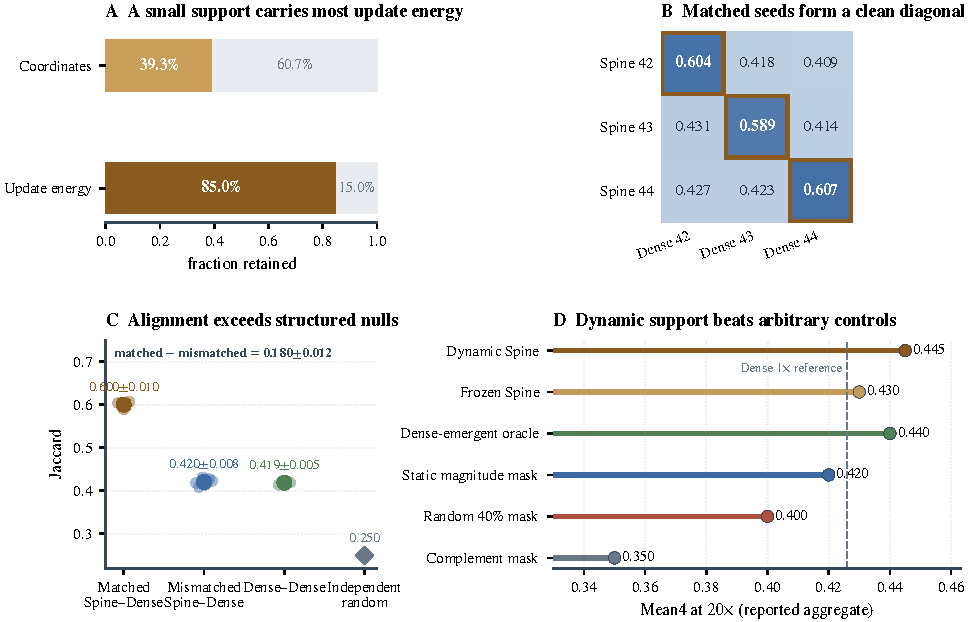
\includegraphics[width=.94\textwidth]{fig_support_evidence.pdf}
\caption{\textbf{The selected support is concentrated, seed-specific, and
non-arbitrary.} (A) The realized 39.3\% support retains 85.0\% of squared adaptive-direction
update norm. (B) The complete Spine--dense cross-seed matrix has a clean
matched diagonal. (C) Matched alignment exceeds both mismatched Spine--dense
and dense--dense structured controls, not only an equal-density random
reference; error bars are descriptive because sets are reused across pairwise
comparisons. (D) At matched reported density and $20\times$, dynamic support
matches the offline oracle numerically and exceeds frozen, static, random, and
complementary controls; points are three-seed means and the manuscript reports
their sample SDs.}
\label{fig:support}
\end{figure*}

\subsection{The direction transfers across algorithms and models}\label{sec:transfer}
The pattern transfers with smaller absolute gains (\cref{tab:transfer}). Under
DAPO on Qwen3-8B, Mean4 changes from $0.440\pm0.0070$ to
$0.455\pm0.0036$ (paired gain $0.015\pm0.0036$). On Qwen3-1.7B, the
three-seed Mean4 changes from $0.36413\pm0.00646$ to
$0.38037\pm0.00760$ (paired gain $0.01624\pm0.00482$). The transfer is not
wholly carried by the two small AIME sets: Mean2 changes
from $0.60257\pm0.00592$ to $0.61108\pm0.00714$, a paired gain of
$0.00851\pm0.00628$, positive in all three seeds. The component result is mixed
rather than universal: Math500 changes by $-0.0013$ while Olympiad changes by
$+0.0184$. On a matched Llama3.1-8B rerun, Mean4 changes from
$0.169\pm0.0062$ to $0.179\pm0.0075$ (paired gain $0.010\pm0.0017$).
The Llama ladder saturates at 10--$20\times$ (both 0.179), unlike the monotonic
Qwen3-8B ladder. The claim is therefore transfer of direction, not an invariant
optimal multiplier.

\begin{table}[t]
\centering
\caption{Three-seed transfer summary. $J$ denotes the mean matched-support
Jaccard; the text reports sample SDs and paired Mean4 gains.}
\label{tab:transfer}
\small\setlength{\tabcolsep}{3.5pt}
\begin{tabular}{lcccc}
\toprule Setting & $J$ & Dense & Recipe & Gain\\
\midrule
Qwen3-8B GRPO & .600 & .426 & .445 & +.019\\
Qwen3-8B DAPO & .572 & .440 & .455 & +.015\\
Qwen3-1.7B & .549 & .364 & .380 & +.016\\
Llama3.1-8B & .513 & .169 & .179 & +.010\\
\bottomrule
\end{tabular}
\end{table}

\begin{table}[t]
\centering
\caption{Qwen3-1.7B benchmark sensitivity across three matched seeds, recomputed
from integer correct/total counts. Entries are mean $\pm$ sample SD; Mean2
excludes AIME24/25 and averages Math500 with Olympiad. The final row is the
paired mean difference.}
\label{tab:qwen17}
\scriptsize\setlength{\tabcolsep}{3.3pt}
\begin{tabular}{lrrrr}
\toprule Condition & Math500 & AIME24 & AIME25 & Olympiad\\
\midrule
Dense & $.742\pm.006$ & $.119\pm.008$ & $.132\pm.007$ & $.463\pm.006$\\
Recipe & $.741\pm.008$ & $.151\pm.009$ & $.149\pm.007$ & $.481\pm.006$\\
$\Delta$ & $-.001$ & $+.031$ & $+.017$ & $+.018$\\
\bottomrule
\end{tabular}
\par\smallskip
\begin{tabular}{lrr}
\toprule Condition & Mean4 & Mean2\\
\midrule
Dense & $.36413\pm.00646$ & $.60257\pm.00592$\\
Recipe & $.38037\pm.00760$ & $.61108\pm.00714$\\
$\Delta$ & $+.01624$ & $+.00851$\\
\bottomrule
\end{tabular}
\end{table}

\subsection{Training overhead is modest and inference remains unchanged}
Across three matched runs per condition, the per-run median RL-step time is
$12.01\pm0.17$\,s for Dense and $13.18\pm0.24$\,s for the recipe. Peak allocated
memory per GPU is $72.2\pm0.9$ and $75.8\pm1.1$\,GiB, respectively. Thus mask
construction adds approximately 9.8\% step time and 4.9\% peak allocated memory
in this implementation. It changes no inference graph and has zero inference
overhead once training is complete. These measurements support feasibility but
are not an end-to-end cluster-cost or hardware-wide benchmark.

\section{Discussion}\label{sec:discussion}
The factorial and controls support a conditional empirical picture.
Down-weighting reduces exposure to a conflict-enriched contribution, while
dynamic top-$k$ avoids applying the amplified global step uniformly. Together
they expand the high-rate operating region under the tested protocol.
Concentrated energy, seed-specific alignment, and density-matched mask controls
argue against arbitrary 40\% selection as a sufficient explanation, while leaving
curvature control, optimality, and the unique causal mechanism unresolved.

Dynamic online selection also differs from an offline oracle. It requires no
completed dense trajectory, yet approaches the oracle aggregate and exceeds
frozen or static supports. This supports adaptation of optimizer-update
coordinates rather than persistent pruning, consistent with the broader role
of changing support in dynamic sparse training
~\cite{evci2020rigl,you2020earlybird}.

The negative-channel result is likewise conditional. Negative samples can
carry useful learning signal~\cite{zhu2025negativereinforcement}, while uniform
penalties can cause likelihood displacement~\cite{deng2025negativegrad}. Our
factorial adds optimizer-scale exposure: attenuation has little effect at the
native rate and becomes protective at the largest rate. The result therefore
identifies the conflict-prone coordinate tail as a candidate contributor to
step-size sensitivity, rather than negative reinforcement as a generally
harmful objective.

\paragraph{Limitations.}
The evidence is limited to three seeds, four mask snapshots over 160 RL steps,
math RLVR, two model families, and one lightly retuned dense condition. The endpoint interval
covers only matched seed variation and is not selection-adjusted. The ladder
ends at $20\times$,
and four mask snapshots cannot reveal a later stability boundary or continuous
support churn. Transfer gains are modest and vary across benchmarks; the tuned
dense arm also shows that part of the degradation is schedule-sensitive.
Longer horizons, broader tasks, and more extensive dense retuning are needed to
map the boundary and scope of the observed operating region; the present claim
is not universal superiority over every retuned dense optimizer.

\section{Conclusion}
A 16-cell, three-seed factorial shows that negative-advantage exposure and
dynamic optimizer-coordinate support jointly shape high-rate RLVR. The
\recipe{} recipe gains 0.0195 Mean4 over dense $1\times$ at the largest tested
rate. Its support concentrates adaptive-direction energy, aligns seed-specifically with
dense-emergent coordinates, and exceeds structured nulls and density-matched
mask controls. These results identify a reproducible, protocol-dependent
high-rate operating region and provide an operational tool for studying its
coordinate structure.

\section*{Reproducibility statement}
The accompanying artifact contains author-attested seed-level result tables,
including integer correct/total records for the primary Qwen3-8B comparison,
and scripts that recompute their rates, means, sample deviations, paired contrasts, and
figures. The release does not present reconstructed manifests, generated hashes,
or synthetic trajectories as raw experimental evidence. Remote raw masks,
checkpoints, and full logs are not redistributed; the released evidence level is
therefore seed-level result reproduction rather than byte-level rerun audit.
Large checkpoints remain available from the corresponding author subject to
storage and license constraints.

\appendix
\section{Learning-rate and state verification}\label{app:audit}
\begin{table}[t]
\centering
\caption{Effective learning rates. Every column agrees within each row.}
\small
\begin{tabular}{ccccc}
\toprule Label & Requested & Optimizer & Scheduler & Logged\\
\midrule
$1\times$&.000005&.000005&.000005&.000005\\
$5\times$&.000025&.000025&.000025&.000025\\
$10\times$&.000050&.000050&.000050&.000050\\
$20\times$&.000100&.000100&.000100&.000100\\
\bottomrule
\end{tabular}
\end{table}
Every new experiment begins at RL step 0 by loading only the designated SFT
model weights. The parent SFT global step is provenance metadata and is not
counted as an RL step. The optimizer and constant scheduler are initialized at
step 0; RL checkpoints and evaluations are recorded at steps 40, 80, 120, and
160. LR assignment, optimizer parameter-group verification, scheduler
verification, and JSONL verification yield zero mismatched runs or steps.
Full-state recovery is reserved for an interruption
of the identical run and restores optimizer, scheduler, trainer-extra, RL-step,
data-position, and RNG states without changing the LR.

\section{Implementation and evaluation contract}\label{app:implementation}
Training uses GRPO with 256 prompts per step and four responses per prompt
(1,024 rollout sequences), a PPO mini-batch of 256, micro-batch size one per
GPU, and eight GPUs. Prompt and response caps are 1,024 and 8,192 tokens.
The objective uses symmetric clipping at 0.2, dual-clip $c=3$, fixed in-loss
low-variance KL with coefficient 0.001, zero entropy coefficient, group-mean
advantage centering, and group-standard-deviation scaling. Dense updates use
AdamW and Top-0.4 updates use SparseAdamW; both use
$(\beta_1,\beta_2)=(0.9,0.999)$, $\epsilon=10^{-8}$, weight decay 0.01,
global gradient clipping at 1.0, a constant LR schedule, and no warmup.
Training rollouts sample four responses at temperature 1.0 and top-$p=1.0$.
Evaluation uses avg@32 at temperature 0.6 and
top-$p=1.0$, with the same 8,192-token response cap. The canonical machine-
readable contract and its digest are included in
\texttt{evaluation\_and\_training\_protocol.json}.

The exploratory tuned-dense diagnostic changes only three optimizer settings:
16 warmup steps, global gradient clipping at 0.5, and $\beta_1=0.8$. Its
three seed-level Mean4 values are released, but the condition is not part of the
factorial or used as a tuned-dense optimum.

\section{Llama exploratory conflict record}\label{app:llama}
The excluded D18 run requested $10^{-4}$ but logged $5\times10^{-6}$ and ended
at step 56 with reward $-1$, AIME accuracy 0, entropy 0.021, response clip ratio
1.0, and collapse. D18b and D18c logged $10^{-4}$ correctly but also collapsed
(steps 63 and 200). These runs are retained as negative evidence and are not
pooled with the matched three-seed rerun in \cref{sec:transfer}.

\section*{CRediT authorship contribution statement}
\textbf{Shikai Li:} Investigation, Writing--original draft.
\textbf{Qingsong Cai:} Writing--review and editing.
\textbf{Rui Shi:} Supervision, Writing--review and editing.

\section*{Declaration of competing interest}
The authors declare no known competing financial interests or personal
relationships that could have influenced the work reported in this paper.

\section*{Declaration of generative AI and AI-assisted technologies in the writing process}
During the preparation of this work, the authors used Cursor and OpenAI Codex
(AI-assisted coding and writing tools) to improve English phrasing and
manuscript organization, assist with \LaTeX{} formatting, and support the
development and review of plotting and consistency-checking code. The authors
reviewed and edited all AI-assisted outputs, independently verified the
references, data-derived quantities, and scientific claims, and take full
responsibility for the content of the published article. These tools were not
used to generate or alter experimental observations or to synthesize image
content. Synthetic schema-testing fixtures used during internal software
validation are excluded from the evidence release and from all reported
results. All tables, the graphical abstract, and the manuscript figures were
produced deterministically from author-verified data using conventional code;
all AI-assisted code was reviewed and executed under author control.

\section*{Data availability}
Result tables, analysis scripts, figure generators, the machine-readable
protocol, and the Advantage Spine implementation are
included in the accompanying open repository
\url{https://github.com/vivia-an/advantage_spine_v1}. Qwen3,
DAPO-Math-17K, AIME25, and VERL are used under Apache-2.0; Llama-3.1 uses its
Community License and Acceptable Use Policy; OlympiadBench uses MIT. Because the
referenced MATH500 and AIME24 cards do not declare a license, the artifact
releases their hashes, identities, counts, and aggregate results but not their
problem text. The public mask evidence consists of author-attested support
metrics rather than the remote raw mask files. The complete
resource matrix is in
\texttt{LICENSE\_AND\_DATA\_USE.md}. Checkpoint redistribution remains subject
to all upstream model and data terms.

\section*{Funding}
This research received no specific grant from public, commercial, or
not-for-profit funding agencies.

\renewcommand{\bibfont}{\scriptsize}
\setlength{\bibsep}{0pt plus 0.2ex}
\bibliographystyle{elsarticle-num}
\bibliography{refs}
\end{document}
